\subsection{Activation functions}
\label{appendix:activations}




\begin{figure*}
    \centering
    \begin{subfigure}[b]{0.4\textwidth}   
        \centering 
        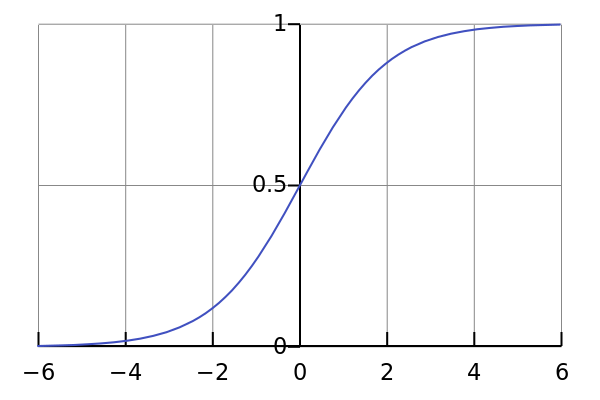
\includegraphics[width=\textwidth]{images/appendix/activations/sigmoid.png}
        \caption[]%
        {{\small Sigmoid activation function.}}    
        \label{fig:appendix_activations_sigmoid}
    \end{subfigure}
    \hfill
    \begin{subfigure}[b]{0.4\textwidth}
        \centering
        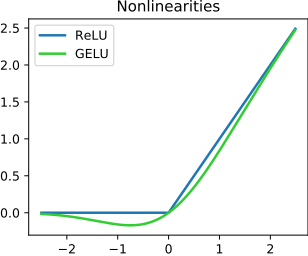
\includegraphics[width=\textwidth]{images/appendix/activations/ReLU_and_GELU.png}
        \caption[]%
        {{\small ReLU and GELU activation functions.}}    
        \label{fig:appendix_activations_relu_and_gelu}
    \end{subfigure}
    \vskip\baselineskip
    \begin{subfigure}[b]{0.4\textwidth}  
        \centering 
        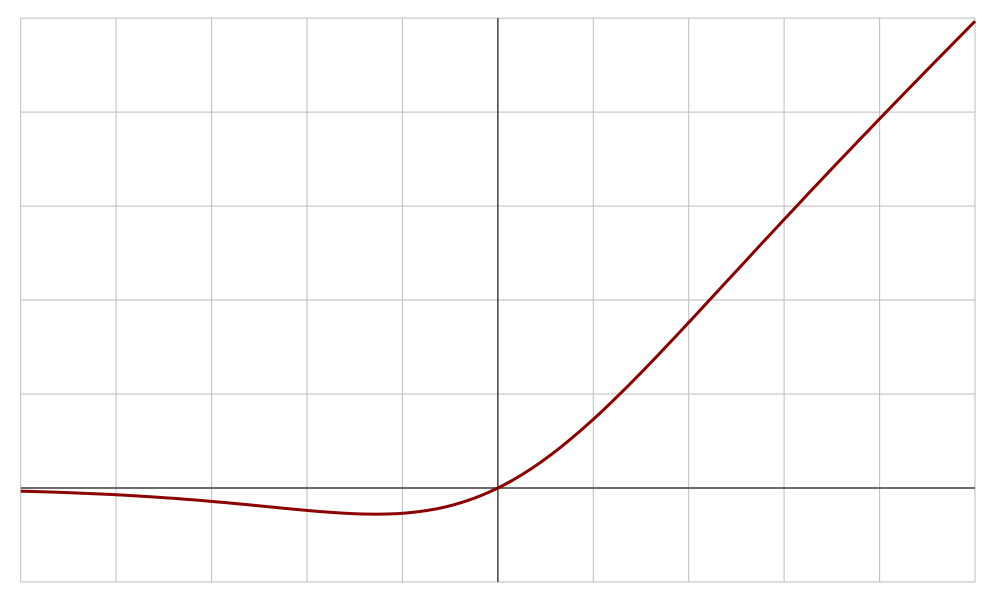
\includegraphics[width=\textwidth]{images/appendix/activations/Swish.png}
        \caption[]%
        {{\small Swish activation function.}}    
        \label{fig:appendix_activations_swish}
    \end{subfigure}
    \hfill
    \begin{subfigure}[b]{0.4\textwidth}   
        \centering 
        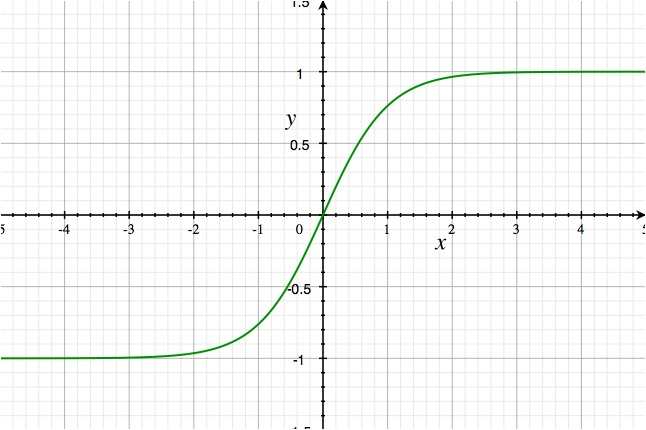
\includegraphics[width=\textwidth]{images/appendix/activations/tanh.jpg}
        \caption[]%
        {{\small Tanh activation function.}}    
        \label{fig:appendix_activations_tanh}
    \end{subfigure}
    \caption []%
    {\small Common activation functions used in deep learning.} 
\end{figure*}






\subsection*{Sigmoid}

Sigmoid (figure \ref{fig:appendix_activations_sigmoid}) is an activation function used in many neural networks. Its one of the most common activation functions. It normalizes the output in the range [0,1] and is usually used in binary classification or logistic regression tasks. In binary classification task it can be used as the last layer of the neural network, which would output a single probability output. It is defined as:

\begin{equation*}
    \sigma(x) = \frac{1}{1 + e^{-x}}
\end{equation*}









\subsection*{ReLU}

ReLU (Rectified Linear Unit) (figure \ref{fig:appendix_activations_relu_and_gelu}) is an activation function used in many neural networks. It is defined as:

\begin{equation*}
    \text{ReLU}(x) = \max(0, x)
\end{equation*}








\subsection*{Softmax}

Softmax is an activation function, usually used in the output layer of a neural network. Its used to compress multiple input values into a range between [0,1] similarly to sigmoid, but softmax can be thought as a probability distribution, where multiple values are mapped to a probability. Softmax is often used in multi-class classification. It is defined as:

\begin{equation*}
    \text{Softmax}(x_i) = \frac{e^{x_i}}{\sum_{j=1}^{n} e^{x_j}}
\end{equation*}

where $x_i$ is the $i$-th element of the input vector $x$ and $n$ is the number of elements in the input vector $x$.






\subsection*{Tanh}

Tanh (figure \ref{fig:appendix_activations_tanh}) is often used in RNNs (Recurrent Neural Networks) and LSTMs (Long Short-Term Memory) gates. Although these models are out of scope in this work, it is still worth mentioning as this activation function is used in many models, such as GANs. The output range is [-1, 1] and its zero centered. It is defined as:

\begin{equation*}
    \tanh(x) = \frac{e^{x} - e^{-x}}{e^{x} + e^{-x}}
\end{equation*}








\subsection*{Swish}

Swish (figure \ref{fig:appendix_activations_swish}) is an activation function used in the Imagen \texttt{ResNetBlock}. It was first introduced in a 2017 paper \cite{ramachandran2017swish} by Google Brain team. It is defined as:

\begin{equation}
    \text{Swish}(x) = x \cdot \sigma(x)
    \label{eq:appendix_activations_swish}
\end{equation}

where $\sigma(x)$ is the sigmoid activation function.

Swish is similar to ReLU activation function but it allows smoother gradients during training, and often it outperforms ReLU in some deep learning tasks.

